\section*{Methods}\label{meth}
We constructed a deterministic compartmental model of heterosexual HIV transmission,
stratified by sex, sexual activity, HIV natural history, and ART cascade of care.
The model includes 8 risk groups,
including higher and lower risk female sex workers (FSW), and higher and lower risk clients of FSW,
plus 4 partnership types, including regular and occasional sex work (Figure~\ref{fig:model}).
We calibrated the model to reflect the HIV epidemic and ART scale-up in Eswatini (\emph{base case}).
We then explored \emph{counterfactual} scenarios in which
ART cascade was reduced among various combinations of risk groups,
and quantified ART prevention impacts by comparing \emph{base case} and \emph{counterfactual} scenarios.
%===================================================================================================
\subsection*{Model Parameterization \& Calibration}\label{meth.param}
Complete details of the model structure, parameterization, and calibration are given in Appendix~\ref{mod}.
\paragraph{HIV}
Our model of HIV natural history included acute infection and stages defined by CD4-count.
We modelled relative rates of infectiousness by stage
as an approximation of viral load \cite{Wawer2005,Boily2009,Donnell2010},
as well as rates of HIV-attributable mortality by stage \cite{Badri2006,Anglaret2012,Mangal2017}.
\paragraph{Risk heterogeneity}
We captured risk heterogeneity through risk-group-level factors, including
group size, average duration in group, STI symptom prevalence, and numbers / types of partnerships per year;
and partnership-level factors, including
assortative mixing, partnership duration, frequency of sex, and levels of condom use.
Table~\ref{tab.het} summarizes key parameter values and sampling distributions related to risk heterogeneity.
We assumed that only condom use varied (increased) over time (Figure~\ref{fig:fit.condom}).
To parameterize higher versus lower risk FSW, we conducted exploratory analysis of
survey data from Swazi FSW in 2011 \cite{Baral2014} and 2014 \cite{EswKP2014} (Appendix~\ref{mod.fsw}).
% TODO ^
We parameterized the remaining risk groups using reported data from national studies in
2006 \cite{SDHS2006}, 2011 \cite{SHIMS1}, and 2016 \cite{SHIMS2}.
We modelled expansion of voluntary medical male circumcision \cite{SHIMS2},
but did not model other interventions (e.g. ongoing pre-exposure prophylaxis scale-up \cite{EswCOP21})
nor non-heterosexual HIV transmission.
\begin{table}
  \centering
  \caption{Model parameters related to risk heterogeneity (* under construction *)}
  \footnotesize
% TODO: update
\begin{tabular}{llrclc}
  \toprule
                          &                                &  \multicolumn{3}{c}{Prior}   &         \\
  \cmidrule(rl){3-5}
  Parameter               & Stratification                 & Mean & (95\% CI)  & Distrib. &  Ref. * \\
  \midrule
  Population size         & FSW of women overall           &  2.8 & (0.6,~6.5) & Beta     &         \\
  (\% of total)           & Clients of men overall         &   30 & (6.0,~70)  & ---      & See~XX  \\
                          & HR FSW of FSW overall          &   20 &    ---     & ---      & Assumed \\
                          & HR clients of clients overall  &   20 &    ---     & ---      & Assumed \\[1ex]
  Duration in group       & HR FSW                         &  3.6 & (1.9,~5.8) & Gamma    & See~XX  \\
  (mean years)            & LR FSW                         &   10 & (9.0,~11)  & Gamma    & See~XX  \\
                          & All clients                    &   10 & (6.0,~15)  & Gamma    &         \\[1ex]
  Relative infectiousness & Acute infection                &  5.3 & (1.0,~13)  & Gamma    &         \\
                          & Any GUD p12m                   &  2.9 & (1.0,~5.7) & Gamma    &         \\[1ex]
  Relative susceptibility & Receptive vaginal sex          & 1.45 & (1.0,~2.0) & Gamma    &         \\
                          & Receptive anal sex             &   10 &    ---     & ---      &         \\
                          & Any GUD p12m: women            &  5.3 & (1.5,~12)  & Gamma    &         \\
                          & Any GUD p12m: men              &  7.7 & (2.0,~18)  & Gamma    &         \\[1ex]
  Any GUD p12m            & LR FSW                         &   16 &  (7,~28)   & Beta     &         \\
  prevalence (\%)         & HR FSW                         &   47 &  (19,~89)  & ---      &         \\
                          & HR clients                     &   12 &  (7,~22)   & ---      &         \\
                          & Everybody else                 &    7 &    ---     & ---      &         \\[1ex]
  Sex acts per            & Main/spousal                   &   78 & (27,~156)  & Gamma    &         \\
  partnership-year        & Casual                         &   30 & (4.4,~82)  & ---      & See~XX  \\
                          & Occasional sex work            &   12 &    ---     & ---      & Assumed \\
                          & Regular sex work               &   31 &  (18,~48)  & Gamma    &         \\[1ex]
  Partnership anal sex    & Main/spousal \& casual         &  5.9 & (0.6,~17)  & Beta     &         \\
  (\% of acts)            & Occasional \& regular sex work &  9.7 & (0.6,~29)  & Beta     &         \\[1ex]
  Condom use in 2020      & Main/spousal                   &   42 &  (31,~54)  & Beta     & See~XX  \\
  (\% of acts protected)  & Casual                         &   69 &  (65,~74)  & Beta     & See~XX  \\
                          & Occasional sex work            &   88 &  (78,~97)  & Beta     & See~XX  \\
                          & Regular sex work               &   79 &  (64,~90)  & Beta     & See~XX  \\
                          & Anal vs vaginal sex            &   77 &  (50,~95)  & Beta     &         \\[1ex]
  Partnerships per year   & LR FSW, occasional sex work    &   49 &  (30,~72)  & Gamma    &         \\
                          & HR FSW, occasional sex work    &   98 & (58,~153)  & ---      &         \\
                          & LR FSW, regular sex work       &  101 & (73,~133)  & Gamma    &         \\
                          & HR FSW, regular sex work       &  151 & (107,~205) & ---      &         \\[1ex]
  Sex work visits         & LR clients                     &   26 &  (11,~50)  & Gamma    &         \\
  per year                & HR clients                     &   89 & (34,~174)  & Gamma    &         \\
  % TODO: mixing!
  \bottomrule
\end{tabular} 
\floatfoot{
  \ffpops;
  p12m: past 12 months.}
  \label{tab.het}
\end{table}
\paragraph{ART cascade}
We modelled rates of HIV diagnosis among people living with HIV as monotonically increasing over time.
We defined a base rate for low/medium activity women,
and constant relative rates for low/medium activity men ($<1$), clients ($<1$), and FSW ($>1$),
reflecting increased access to HIV testing via antenatal care among women versus men,
and enhanced screening among FSW \cite{Baral2014}.
We modelled ART initiation similarly except:
the relative rate for ART initiation among FSW was $<1$,
reflecting unique barriers to uptake and engagement in care \cite{Mountain2014sr}; and
we defined an additional relative rate by CD4 count ($\le1$)
to reflect historical ART eligibility criteria \cite{NERCHA2018}.
We modelled viral suppression using a fixed rate for all groups,
corresponding to an average of 4 months on ART \cite{Mujugira2016}.
We modelled treatment failure / discontinuation with a single monotonically decreasing rate
applied to all risk groups in the base case,
reflecting improving treatment success / retention over time \cite{NERCHA2014}.
Individuals with treatment failure / discontinuation could re-initiate ART at a fixed rate,
reflecting re-engagement in care or detection of treatment failure and initiation of alternative regimens.
We modelled rapid CD4 recovery during the first 4 months of ART,
followed by slower recovery while virally suppressed \cite{Battegay2006,Lawn2006,Gabillard2013}.
We modelled reduced HIV-attributable mortality among individuals on ART,
in addition to mortality benefits of CD4 recovery.
\paragraph{Calibration}
We calibrated the model to reflect
available data from Eswatini on HIV prevalence, HIV incidence, and ART cascade of care,
stratified by risk groups (Appendix~\ref{mod.cal}) \cite{SDHS2006,SHIMS1,SHIMS2,Baral2014,EswKP2014}.
% TODO: finish
%===================================================================================================
\subsection*{Scenarios \& Analysis}\label{meth.obj}
%---------------------------------------------------------------------------------------------------
\subsubsection*{Objective~1: Influence of cascade differences between risk groups}\label{meth.obj.1}
For Objective~\ref{obj:1},
We defined the \emph{base case} scenario to reflect
observed cascade scale-up in Eswatini, reaching \cashi by 2020 \cite{AIDSinfo}.
Next, we defined 4 \emph{counterfactual} scenarios in which overall viral suppression was lower,
such that the population overall reached \casmd by 2020,
reflecting approximate trends in SSA cascades prior to universal ART \cite{AIDSinfo}.
In these counterfactual scenarios, we reduced cascade progression
among specific risk groups in different combinations:
FSW, clients, and/or the remaining population (``lower risk'').
We reduced cascade progression by calibrating and applying
a constant relative scaling factor ``$R$'' to group-specific rates of:
diagnosis ($R_d \in [0,1]$),
treatment initiation ($R_t \in [0,1]$), and
treatment failure / discontinuation ($R_u \in [1,20]$).
When FSW and/or clients had reduced cascade, we calibrated their $R$s so that
these populations achieved approximately \caslo by 2020.
By contrast, we calibrated $R$s for the lower risk population so that
the Swati population \emph{overall} achieved \casmd in all 4 counterfactual scenarios,
thus ensuring that a consistent proportion of the population overall
experienced reduced viral suppression.
Table~\ref{tab:art.scenarios} summarizes these scenarios, while
Figure~\ref{fig:obj.1.cascade} plots the modelled cascades over time.
When cascade rates among FSW and/or clients were unchanged from the base case,
the cascade these groups achieved could be lower than \cashi
due to risk group turnover and higher incidence.
All cascades continued to increase beyond 2020 due to assumed fixed rates of
diagnosis, treatment initiation, and treatment failure / discontinuation thereafter.
\begin{table}
  \centering
  \caption{Modelling scenarios for Objective~\ref{obj:art.1} defined by 2020 calibration targets}
  \label{tab:art.scenarios}
  \begin{tabular}{lCCCccc}
  \toprule
  & \multicolumn{3}{c}{ART cascade in 2020\tn{a}} 
  & \multicolumn{3}{c}{Re-scaled cascade rates\tn{b}} \\
  \cmidrule(rl){2-4}\cmidrule(rl){5-7}
  Scenario                                   &   FSW    & Clients  & Overall  & FSW & Clients & LR  \\
  \midrule
  \emph{Base Case}                           & 95-95-95 &    ---   & 95-95-95 & --- &   ---   & --- \\
  \emph{Leave Behind: FSW}                   & 40-60-80 &    ---   & 60-80-80 & \By &   \Bn   & \By \\
  \emph{Leave Behind: Clients}               &    ---   & 40-60-80 & 60-80-80 & \Bn &   \By   & \By \\
  \emph{Leave Behind: FSW \& Clients}        & 40-60-80 & 40-60-80 & 60-80-80 & \By &   \By   & \By \\
  \emph{Leave Behind: Neither}               &    ---   &    ---   & 60-80-80 & \Bn &   \Bn   & \By \\
  \bottomrule
\end{tabular}\floatfoot
\tnt[a]{Cascade: \% diagnosed among HIV+; \% on ART among diagnosed; \% virally suppressed among on ART};
\tnt[b]{Rates of: diagnosis; ART initiation; treatment failure}.
% TODO: explain counterfactual scenario re-fitting details?
\end{table}
% TODO: (~) create figure of these cascades like CROI poster
\par
We quantified ART prevention impacts via relative
cumulative additional infections (CAI) and additional incidence rate (AIR)
in the counterfactual scenarios ($k$) \vs the base case ($0$),
over multiple time horizons up to 2030, starting from $t_0 = 2000$:
\begin{equation}
  \txn{CAI, AIR}\,(t) = \frac{\Omega_{k}(t) - \Omega_{0}(t)}{\Omega_{0}(t)}
  ,\qquad \Omega(t) =
  \begin{cases}
    ~\int_{t_0}^{t}\!\Lambda(\tau)\,d\tau & \txn{CAI} \\
    ~\lambda(t) & \txn{AIR}
  \end{cases}
\end{equation} where:
$\Lambda$ denotes absolute numbers of infections per year, and
$\lambda$ denotes incidence rate per susceptible per year.
For each scenario, we computed these outcomes (CAI and AIR) for each model fit $j$,
and reported median (95\% CI) values across model fits, reflecting uncertainty.
%---------------------------------------------------------------------------------------------------
\subsubsection*{Objective~2: Conditions that maximize the influence of cascade differences}\label{meth.obj.2}
For Objective~\ref{obj:2}, we estimated via regression:
the effects of lower cascade among certain risk groups on relative CAI and AIR,
plus potential effect modification by epidemic conditions.
The hypothesized causal effets are illustrated
as a directed acyclic graph in Figure~\ref{fig:obj.2.dag},
and the synthetic data generation processes and variable definitions are as follows.
\par
For this regression analysis, we obtained 10,000 samples.
We explored a wider range of counterfactual scenarios \vs Objective~\ref{obj:1}
by randomly sampling the relative rates for
diagnosis and treatment initiation $R_d, R_t \sim \opname{Beta}(\alpha=3.5,\beta=1.9)$
and treatment failure $R_u \sim \opname{Gamma}(\alpha=3.4,\beta=1.9)$
% TODO ^ param values
for each of: FSW, clients, and the remaining lower risk population (9~total values).
These sampling distributions had 95\%~CI: (0.25,~0.95) and (1.5,~15), respectively,
and were chosen to obtain cascades in 2020 spanning
approximately \mbox{60-60-90} through \mbox{90-90-95} (Figure~\ref{fig:obj.2.cascade}). % MAN
For each of $N_f = 1000$ model fits, we generated $N_k = 10$ counterfactual scenarios per fit
via random relative rates ``$R$'' via Latin hypercube sampling,
yielding $N_f N_k = {}$10,000 total counterfactual samples for the regression.
\begin{figure}
  \centering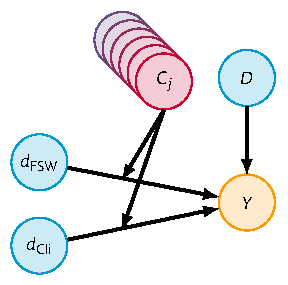
\includegraphics[scale=1]{art.dag.obj.2}
  \caption{Directed acyclic graph (DAG) for inferring
    the epidemic conditions under which
    differential viral suppression across risk groups matters most}
  \label{fig:art.2.dag}
  \floatfoot{
    $Y$: cumulative additional infections (CAI) or additional incidence rate (AIR) by 2030;
    $D$: difference in population-overall viral unsuppression
      in counterfactual \vs base case scenario;
    $d_i$: difference in group-$i$-specific viral unsuppression
      \vs population overall within counterfactual scenario;
    $C_j$: epidemic conditions (effect modifiers of $d_i$).}
\end{figure}
\par
For each of these 10,000 samples, we defined
relative CAI and AIR by 2030 \vs the base case, as in Objective~\ref{obj:1}.
For each sample, we further defined
$U_{fki}$ for risk groups $i \in \{\tdef{1}{FSW}, \tdef{2}{clients}, \tdef{*}{overall}\}$
as the proportions virally unsuppressed among people living with HIV by 2020,
reflecting a summary measure of ART cascade gaps.
Using $U_{fki}$, we defined the main regression predictors as:
$D_{fk} = U_{fk*} - U_{f0*} > 0$, reflecting differences in
\emph{population-overall} viral unsuppression in sample $k \in [1,10]$
\vs the base case (denoted $k = 0$); and
$d_{fki} = U_{fki} - U_{fk*} \lessgtr 0$, reflecting differences in
\emph{group-$i$-specific} viral unsuppression in sample $k$
\vs the population overall in sample $k$ --- \ie disproportionate unsuppression.
\par
Next, we defined the following measures of epidemic conditions ($C_{fj}$) related to sex work,
as hypothesized modifiers of the effect of disproportionate unsuppression on relative CAI and RAI:
FSW and client population sizes (\% of population overall);
average rate of turnover among FSW and clients (per year, reciprocal of duration selling / buying sex); and
HIV incidence ratios in the year 2000 among FSW \vs other women, and among clients \vs other men.
For these measures, we combined higher and lower risk FSW, and likewise higher and lower risk clients.
We used HIV incidence ratios in 2000 to reflect summary measures of risk heterogeneity prior to ART,
as compared to including all modelled risk factors for HIV acquisition,
which could lead to overfitting and improper inference due to effect mediation.
\par
Finally, we defined a general linear model for each outcome (CAI, AIR) as:
\begin{equation}\label{eq:art.glm}
  \txn{CAI, AIR} = \beta_0\,D
                 + \sum_i \beta_i\,d_i
                 + \sum_{ij} \beta_{ij}\,d_i\,C_j
\end{equation}
such that each outcome was modelled as a sum of the effects of:
differential population-level unsuppression in the counterfactual \vs the base scenario ($D$);
differential unsuppression among FSW and clients
\vs the population overall within the counterfactual scenario ($d_i$); and
effect modification of $d_i$ by epidemic conditions ($C_j$).
The model does not include an intercept because if $D = d_i = 0$,
then we expect $\txn{CAI} = \txn{AIR} = 0$.
We fitted this model for each outcome using generalized estimating equations \cite{Halekoh2006}
to control for repeated use of each model fit $f$.
We standardized all model variables ($D$, $d_i$, $C_j$) via
$\hat{x} = (x - \txn{mean}(x)) / \txn{SD}(x)$
to avoid issues of different variable scales and collinearity in interaction terms.
This standardization does not imply that
regression coefficient magnitudes can be compared to indicate variable ``importance'',
because the standardization applied to each variable is driven
by the variance before standardization
--- in this case reflecting arbitrary ranges ($D$, $d_i$) or uncertainty in calibration ($C_j$).%
\footnote{We verified that results were qualitatively the same using
  $\hat{x} = (x - \txn{median}(x)) / \txn{IQR}(x)$.
  For further discussion on interpretation of standardized regression coefficients,
  see also: \hreftt{stats.stackexchange.com/questions/29781} and links therein.}
Rather, effect sizes can be interpreted as:
the expected change in outcome per standard deviation change in the variable.
